% Preview source code

%% LyX 2.0.0beta3 created this file.  For more info, see http://www.lyx.org/.
%% Do not edit unless you really know what you are doing.
\documentclass[a4paper,11pt,oneside,english]{article}
\setcounter{secnumdepth}{3}
\setcounter{tocdepth}{3}
\usepackage[T1]{fontenc}
\usepackage[utf8]{inputenc}
\usepackage[margin=2.5cm]{geometry}
\usepackage{babel}
\usepackage{listings}
\usepackage{graphicx,subcaption}
\usepackage{colortbl}
\usepackage[unicode=true,pdfusetitle,
 bookmarks=true,bookmarksnumbered=true,bookmarksopen=false,
 breaklinks=false,pdfborder={0 0 0},backref=section,colorlinks=true]
 {hyperref}
\hypersetup{pdfstartview=FitH,pdfpagelayout=SinglePage}

\newcommand{\cubit}{\textsc{Cubit}}
\newcommand{\geocubit}{\textsc{GeoCubit}}
\newcommand{\specfem}{\textsc{Specfem3D}}

\definecolor{codebg}{RGB}{238,238,238}
\definecolor{codeframe}{RGB}{204,204,204}
\lstset{
  % The bash style works pretty well for cfg files as well.
  language=bash,
  basicstyle=\small\ttfamily,
  breakatwhitespace=true,
  breaklines=true,
  escapechar=\@,
  backgroundcolor=\color{codebg},
  frame=single,
  framesep=10pt,
  rulecolor=\color{codeframe}
}

\begin{document}

\title{\geocubit\ User Manual}
\author{Emanuele Casarotti}

\maketitle

\tableofcontents

\clearpage
\section{Why?}

\geocubit\ is a Python library wrapping around the \href{http://cubit.sandia.gov} {\cubit}
Python Interface and it aims to facilitate the meshing
process in some common problems in seismic wave propagation.
In particular, it is focused on the meshing requests of \specfem\ and it is helpful for such tedious tasks as:
%
\begin{itemize}
\item Creation of geophysical surfaces and volumes (ex. topography).
\item Mesh of layered volumes with hexahedral.
\item Creation of an anisotropic mesh suitable for cases where some alluvial
basin (or slow velocity zones) are present.
\item It can be used as a serial or parallel process. The parallel meshing
capabilities are fundamental for large geophysical problems (ex. mesh
of Southern California using SRTM topography).
\end{itemize}

\geocubit\ can be used inside the graphical interface of \cubit\ (i.e.
as a Python object in the script tab) or as unix command. We refer to the
\cubit\ help appendix for more information about the Python interface.

\clearpage
\section{First Steps}


\subsection{Requirements}

The minimum requirements for using \geocubit\ are:
%
\begin{itemize}
\item \href{http://cubit.sandia.gov} {\cubit\ 12.2}
\item \href{http://downloads.sourceforge.net/numpy} {NumPy 1.0+}
\item \href{http://www.python.org} {Python 2.5}
 (strictly! it depends on the \cubit\ library that refers to this version of Python)
\end{itemize}
%
and for using the parallel meshing capabilities:
%
\begin{itemize}
\item \href{http://downloads.sourceforge.net/pympi/pyMPI-2.4b4.tar.gz} {pyMPI}
\end{itemize}

\subsection{Installation}

For installing, download the code and type in the GEOCUBIT directory:
%
\begin{lstlisting}
python2.5 setup.py install
\end{lstlisting}
%
and check that the following variables are set:
%
\begin{lstlisting}
CUBITDIR="/usr/local/CUBIT"
CUBITLIB="$CUBITDIR/bin:$CUBITDIR/structure:$CUBITDIR/components"
PYTHONPATH="$CUBITDIR/components/cubit:$CUBITDIR/structure:$CUBITDIR/bin"
LD_LIBRARY_PATH="$CUBITDIR/bin"
PATH="$CUBITDIR/bin:$CUBITDIR/components/cubit"
\end{lstlisting}


\clearpage
\section{Using \geocubit\ from the Command Line}

\subsection{Utilities}

\begin{itemize}
\item Checking the configuration of the libraries and dependencies:
\begin{lstlisting}
GEOCUBIT.py --chklib
\end{lstlisting}

\item Checking the parameter file:
\begin{lstlisting}
GEOCUBIT.py --chkcfg --cfg=[file]
\end{lstlisting}
\end{itemize}

\subsection{Create Geometry}

\subsubsection{Surfaces}

\begin{itemize}
\item Creating acis surfaces using a parameter file:
\begin{lstlisting}
 GEOCUBIT.py --build_surface --cfg=[filename]
\end{lstlisting}
\end{itemize}

\begin{itemize}
\item Creating a surface from regular ascii grid or ascii lines that define a "skin":
\begin{lstlisting}
 GEOCUBIT.py --surface=[file] (--regulargrid=[opts] | --skin=[opts])
\end{lstlisting}
\end{itemize}

\subsubsection{Volumes}

\begin{itemize}
\item \emph{Serial} command: creating \cubit\ volumes using a parameter file:
\begin{lstlisting}
GEOCUBIT.py --surface=[file] (--regulargrid=[opts] | --skin=[opts])
\end{lstlisting}
\end{itemize}

\begin{itemize}
\item \emph{Parallel} command: creating \cubit\ volumes using a parameter file:
\begin{lstlisting}
mpirun -n [numproc] pyMPI GEOCUBIT.py --build_volume --cfg=[file]
\end{lstlisting}


\begin{figure}[htbp]
  \centering
  \begin{subfigure}{0.45\textwidth}
    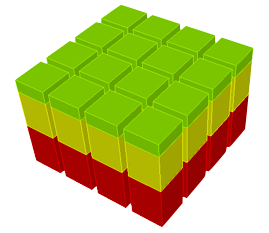
\includegraphics[width=\textwidth,keepaspectratio]{media/geocubitmanual_grid2.jpg}
    \caption{Volume divided in slices.}
    \label{fig:vol}
  \end{subfigure}
  \begin{subfigure}{0.45\textwidth}
    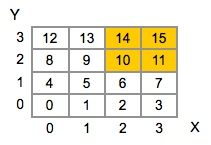
\includegraphics[width=\textwidth,keepaspectratio]{media/geocubitmanual_grid.jpg}
    \caption{Parallel map of the IDs for volume in \autoref{fig:vol} divided in 16 slices (4 along x-axis and 4 along y-axis).}
    \label{fig:table}
  \end{subfigure}
  \caption{Volume slicing.}
  \label{fig:grid}
\end{figure}

In this parallel application, the volume is separated in $N$ slices, each one is assigned at a single process and one file for each slice is created (see \autoref{fig:grid} as example).
\end{itemize}

\subsection{Meshing}

\begin{itemize}
\item \emph{Serial} command: building a volume and meshing it.
\begin{lstlisting}
GEOCUBIT.py --build_volume --mesh --cfg=[file] (--id_proc=n)
\end{lstlisting}

\item \emph{Serial} command: meshing a volume
\begin{lstlisting}
GEOCUBIT.py --mesh --cfg=[file] (--id_proc=[n, def=0])
\end{lstlisting}

{\footnotesize note: without the \lstinline|--build_volume| flag the script recall an old "\lstinline|geometry_vol_[id_proc].cub|" file}

\item \emph{Parallel} command: meshing a volume from a parameter file
\begin{lstlisting}
mpirun -n [nproc] pyMPI GEOCUBIT.py --build_volume --mesh --cfg=[file]
\end{lstlisting}
\end{itemize}

\subsection{Finalizing and Exporting}

It is possible to collect, merge, set the absorbing boundary conditions and to export the resulting mesh in a format readable by \specfem.
\begin{itemize}
\item
Collecting some \cubit\ files, setting the absorbing boundary conditions and merging in a single free mesh cubitfile
\begin{lstlisting}
GEOCUBIT.py --collect --merge --meshfiles=[files] --cpux=N --cpuy=N (--rangecpux=[cpuxmin,cpuxmax] --rangecpuy=[cpuymin,cpuymax])
\end{lstlisting}

\lstinline{cpux, cpuy} set the number of cpus used for creating the mesh files; \lstinline{rangecpux} and \lstinline{rangecpuy} set the range of slices that are used in the mesh.

Following the example in \autoref{fig:grid}, the parameters \lstinline{--cpux=4 --cpuy=4 --rangecpux=1,2 --rangecpuy=2,3} select the slices with id $10, 11, 14, 15$. Only these slices are going to be collected and merged with the appropriate absorbing boundary conditions.

\item Collecting a single free mesh cubitfile and refine the hex inside some curves (ex. alluvial basin, \autoref{fig:refcurve})
\begin{lstlisting}
GEOCUBIT.py --collect --meshfiles=[list of files] --curverefining=[file]
\end{lstlisting}

{\footnotesize note: the curves must be stored in acis format (sat) and must be closed.}

\begin{figure}[htbp]
\center
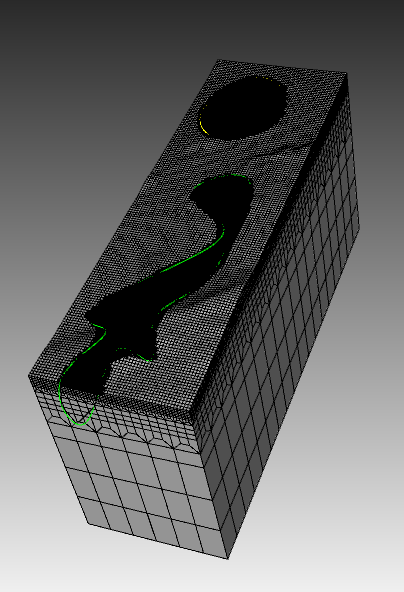
\includegraphics[height=0.4\textheight,keepaspectratio]{media/refcurve_1.png}%
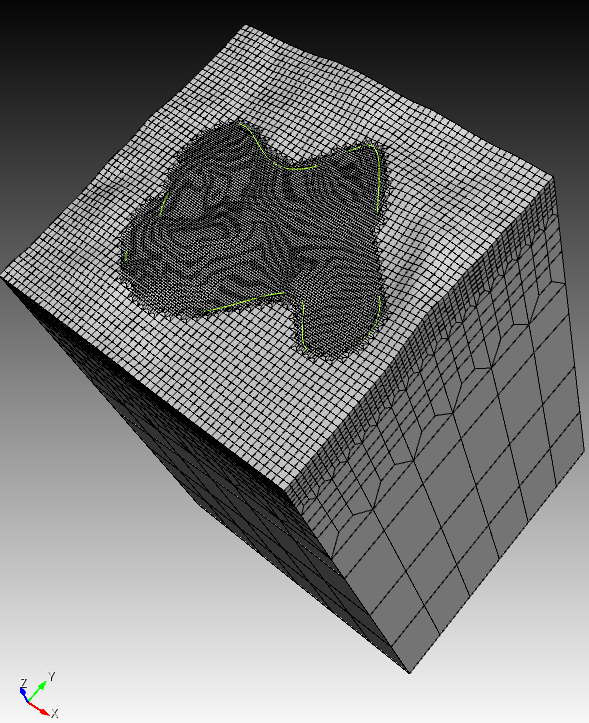
\includegraphics[height=0.4\textheight,keepaspectratio]{media/refcurve_2.png}%
\caption{An alluvial basin example.}

\label{fig:refcurve}
\end{figure}

\item Exporting a \cubit\ mesh file to a \specfem\ mesh
\begin{lstlisting}
GEOCUBIT.py --export2SPECFEM3D=[output directory] --meshfiles=[filename] (--listblock=[list of @\cubit@ blocks] --listflag=[list of specfem3d flags])
\end{lstlisting}

If required, it is possible to assign personalized flags to each block using \lstinline{--listblock} and the corresponding listflag (for example: \lstinline{--listblock=3,4 --listflag=1,-1})
\end{itemize}

\clearpage
\section{\geocubit\ and \cubit\ Graphical Interface}

In the Python script tab of \cubit\ GUI, type:

\begin{lstlisting}
>f="volume.cfg" # store the name of the configuration file, see next section

>from geocubitlib import volumes # load the @\geocubit@ modules
>from geocubitlib import mesh_volume
>from geocubitlib import exportlib

volumes.volumes(f)  # create the volumes, the parameters are stored in the cfg file
mesh_volume.mesh(f) # mesh the volume

exportlib.collect()                # set the boundary conditions, see @\specfem@ manual
exportlib.e2SEM(outdir="./output") # save the mesh in the @\specfem@ format
\end{lstlisting}

See the \lstinline|media/iterative.mov| for a live example.

\section{Examples of Configuration Files}

In the current section a few configuration files will be described. Please see the files in the examples directory of the \geocubit\ distribution for reference.

\subsection{General Options}

A cfg file has a format similar to ini windows files.
They are divided in \lstinline{[sections]}. There is no order in the position or in the name of the sections.

Generally, the parameters that control the general options are in the first section, called \lstinline{[cubit.options]} and \lstinline{[simulation.cpu_parameters]}. For example:

\begin{lstlisting}
[cubit.options]
cubit_info=off             # turn on/off the information of the @\cubit@ command
echo_info=off              # turn on/off the echo of the @\cubit@ command
cubit_info=off             # turn on/off the @\cubit@ journaling
echo_info=off              # turn on/off the @\cubit@ error journaling
working_dir=tmp            # set the working directory
output_dir=output          # set the output directory
save_geometry_cubit = True # true if it saves the geometry files
save_surface_cubit = False # true if it saves the surfaces in a @\cubit@ files
export_exodus_mesh = True  # true if it saves the mesh also in exodus format. The default is the @\cubit@ format (cub), that contains both the geometry and the meshing information. In case of complex geometry, the cub file could be enormous and a more light exodus file become important.

[simulation.cpu_parameters]
nodes = 1  # number of nodes/process
\end{lstlisting}

{\footnotesize note: Usually the \lstinline|*_info| options are turned off by default for improving the performance.}

\subsection{Creating a Topographic Surface}

{\footnotesize See stromboli.cfg, execute with: \lstinline|GEOCUBIT.py --build_surface --cfg=./example/stromboli.cfg|.}

\geocubit\ is able to create a topographic surface based upon the \cubit\ command \lstinline|create skin curve| and \lstinline|create surface net| (\autoref{fig:surfacetype}). See the \cubit\ manual for details.

\begin{lstlisting}
[geometry.surfaces]
nsurf = 2 # number of surfaces that will be created

[surface1.parameters]
name=example/data/stromboli.xyz # the name of the file defining the surface
surf_type=skin # the type of surface: @\texttt{skin}@: the file is a sequence of parallel points that span the surface in the order described by the following direction parameters; @\texttt{regular\_grid}@: the points are structured distributed. See @\cubit@ Manual for details (skin surface and net surface)
unit_surf = utm # unit of the points, @\texttt{utm}@ or @\texttt{geo}@ (geographical) coordinates
directionx = 0 # if surf_type=skin: @\texttt{directionx}@ and @\texttt{directiony}@ define how the points span the surface
directiony = 1
step = 1 # the script creates a vertex each @\texttt{step}@ points: in this case @\texttt{step=1}@ means a vertex for all the points

[surface2.parameters] # note the different number of surface in the section name
name=./examples/surfaces/topo.dat # the name of the file defining the surface
surf_type=regular_grid # the type of surface: @\texttt{skin}@: the file is a sequence of parallel points that span the surface in the order described by the following direction parameters; @\texttt{regular\_grid}@: the points are structured distributed. See see @\cubit@ Manual for details (skin surface and net surface)
unit_surf= geo # unit of the points, @\texttt{utm}@ or @\texttt{geo}@ (geographical) coordinates
nx=5 # In case of @\texttt{regular\_grid}@: @\texttt{nx}@ and @\texttt{ny}@ are the number of points along x and y direction.
ny=5
\end{lstlisting}

\begin{figure}[htbp]
  \centering
  \begin{subfigure}{0.4\textwidth}
    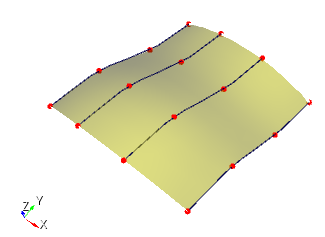
\includegraphics[width=\textwidth,keepaspectratio]{media/skinsurface.png}
    \caption{Skin topography, \texttt{directionx=0} and \texttt{directiony=1}}
    \label{fig:skin}
  \end{subfigure}
  \begin{subfigure}{0.4\textwidth}
    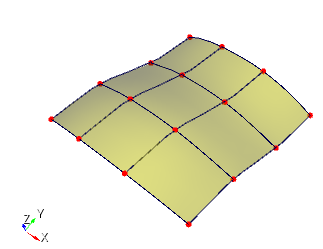
\includegraphics[width=\textwidth,keepaspectratio]{media/netsurface.png}
    \caption{Topography from a net of structured distributed points, \texttt{nx=4} and \texttt{ny=4}}
    \label{fig:net}
  \end{subfigure}

  \begin{subfigure}{0.4\textwidth}
    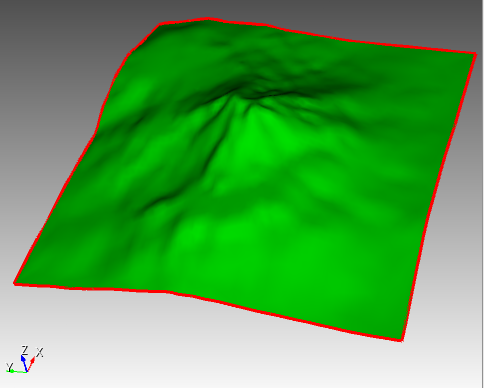
\includegraphics[width=\textwidth,keepaspectratio]{media/strombolisurface.png}
    \caption{Topography of Stromboli volcano (Italy) using the net surface method.}
    \label{fig:stromboli}
  \end{subfigure}
  \caption{Two methods of creating a topographic surface in \geocubit.}
  \label{fig:surfacetype}
\end{figure}


\subsection{Creating and Meshing a Volume}

{\footnotesize see volume.cfg, for executioning: \lstinline|GEOCUBIT.py --build_volume --mesh --cfg=./example/volume.cfg|}

The example is for a volume with topography with dimension of the hexahedra increasing with depth by means of a refinement layer (\autoref{fig:volume}).

\begin{figure}[htbp]
\centering
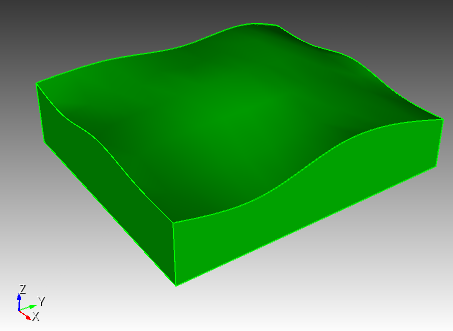
\includegraphics[height=0.24\textheight,keepaspectratio]{media/geometryvolume.png}%
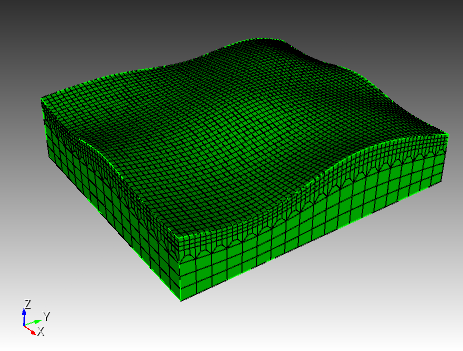
\includegraphics[height=0.24\textheight,keepaspectratio]{media/meshvolume.png}%
\caption{Mesh of a simple volume}

\label{fig:volume}
\end{figure}

\begin{lstlisting}
[geometry.volumes]
volume_type = layercake_volume_ascii_regulargrid_regularmap
latitude_min                    = 13.879
latitude_max                    = 14.279
longitude_min                   = 40.619
longitude_max                   = 40.969
nx = 5
ny = 5
unit                            = geo

[geometry.volumes.layercake]
nz = 2
bottomflat = True
depth_bottom = -7000
filename = ./example/topo.dat
geometry_format=ascii
\end{lstlisting}

\begin{description}
\item[nz] is the number of the horizontal surfaces in the volume (in this case: topography and bottom).
\item[bottomflat] is \lstinline|True| if the bottom is flat.
\item[depth\_bottom] is the depth of the bottom.
\item[filename] is a list of files. Each one defines a surface (in this case there is only the topography file in a \lstinline|regular_grid| format).
\item[geometry\_format] is set to \lstinline|ascii| since the definition of the surfaces comes from ASCII files (structured xyz points).
\end{description}

\begin{lstlisting}
[meshing]
map_meshing_type=regularmap
iv_interval=5, # if only one value is present, append the comma
size=2000
or_mesh_scheme=map
ntripl=1
tripl=2, # if only one value is present, append the comma
smoothing=False
\end{lstlisting}

The \lstinline|[meshing]| section contains the parameters requested for the meshing process.

\begin{description}
\item[map\_meshing\_type] sets the meshing scheme and is \lstinline|regularmap| by default (other schemes are in preliminary phase).
\item[iv\_interval] sets the number of "horizontal" hex sheets for each layer.
\item[size] is the dimension of hexahedral (horizontally).
\item[or\_mesh\_scheme] is the meshing scheme for the topography (\lstinline|map| or \lstinline|pave| are possible, see the \cubit\ manual for more information).
\item[ntripl] is the number of tripling layer in the mesh (in this case 1).
\item[tripl] means in this case that the refinement layer is located at the second surface (the topography). The surfaces are ordered from the bottom (surface 1) to the top (surface 2).
\item[smoothing] performs the smoothing command in \cubit.
\end{description}


\subsection{Layered Volume and Mesh for Central Italy (in Parallel)}

In the example abruzzo.cfg, the layers are 2. For execution, type: \lstinline|mpirun -n 150 GEOCUBIT.py --build_volume --mesh --cfg=./example/abruzzo.cfg|.

Comparing the previous cfg files, there are few modifications:
%
\begin{lstlisting}
. . .
nz = 3
. . .
filename = example/data/moho_int.xyz,example/data/topo.xyz
. . .
iv_interval=8,8 (one value for each layer)
. . .
refinement_depth=1,
\end{lstlisting}

The volume has \lstinline|nz=3| interfaces: bottom, moho, and topography. The bottom is flat and its z-coordinate position is set by \lstinline|depth_bottom|.
The name of the files that storage the data for the other interfaces are listed in \texttt{filename}.
The interfaces defines 2 geological layers. Each layer has \lstinline|iv_interval=8| "horizontal" hex sheets. There is only a refinement and it is set in the \lstinline|refinement_depth=1| hex sheet, i.e just below the topography (\lstinline|refinement_depth=8| means just below the moho).


\subsection{Creation of a Regular Mesh}

In the example grid.cfg, the layers are 3. For execution, type: \lstinline|GEOCUBIT.py --build_volume --mesh --cfg=./example/grid.cfg|.

In this example we create a simple layercake box \lstinline|geometry_format=regmesh| with 3 layers at depth defined by \lstinline|zdepth=-7000,-3000,-600,0|. The initial mesh has hex with horizontal size \lstinline|size=2000| and the numbers of vertical hex sheets is \lstinline|iv_interval=3,1,1| respectively for the bottom, middle and top layer. We include a refinement layer (\lstinline|ntripl=1|) at \lstinline|tripl=2,| interface (the second from the bottom). Since the refinement occurs on the vertical direction, the vertical dimensions of the hexes in the top layer is too small and the quality of the mesh decreases. \lstinline|coarsening_top_layer=True| remesh the top layer and the number of vertical hex sheet in the vertical is defined by \lstinline|actual_vertical_interval_top_layer=1|. (see \autoref{fig:regrid})

\begin{figure}[htbp]
  \centering
  \begin{subfigure}{0.45\textwidth}
    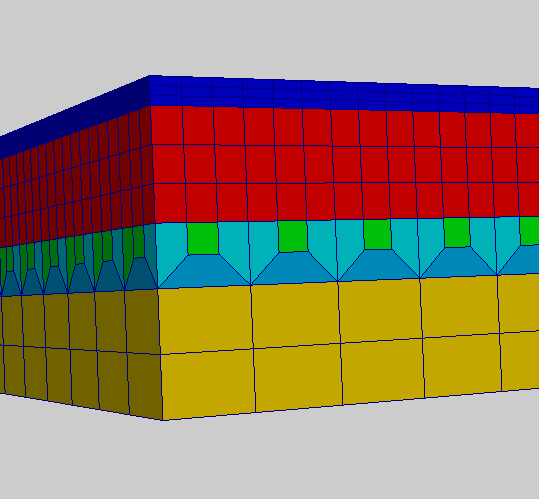
\includegraphics[width=\textwidth,keepaspectratio]{media/regrid.png}
    \caption{Mesh with \lstinline|coarsening_top_layer=False|}
    \label{fig:regrid_nocoarse}
  \end{subfigure}
  \begin{subfigure}{0.45\textwidth}
    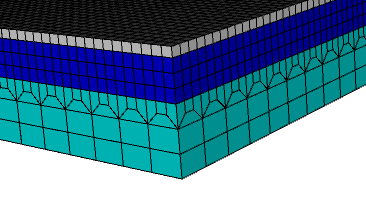
\includegraphics[width=\textwidth,keepaspectratio]{media/regrid_coarse.png}
    \caption{Mesh with \lstinline|coarsening_top_layer=True|. The top layer is remeshed with \lstinline|actual_vertical_interval_top_layer=1| vertical hex sheet.}
    \label{fig:regrid_coarse}
  \end{subfigure}
  \caption{Regular mesh with one tripling layer.}
  \label{fig:regrid}
\end{figure}


\subsection{TODO: Mesh for Southern California}
Mesh with high number of hexes and high resolution topography. Mesh in Parallel.

TO DO


\subsection{TODO: Mesh for Santa Monica Overtrust}
Using part of the mesh for Southern California, stitching together several slices. 

TO DO

\subsection{TODO: Grouping Hexes with Different Resolved Periods}

Checking the stability
For execution type: \lstinline|GEOCUBIT.py --meshfiles=[filename] --stability (--tomofile=[tomographic file]/--vp=[vp text value] --vs=[vs text value])|.

Or in the script tab of the \cubit\ GUI, type:

\begin{lstlisting}
>from geocubitlib.hex_metric import SEM_stability_3D # load the @\geocubit@ modules
>mesh=SEM_stability_3D()
>mesh.check_simulation_parameter(vp_static=vp,vs_static=vs) # test the mesh against some homogeneous velocity model
# or
>mesh.check_simulation_parameter(tomofile=tomofile) # test the mesh against a tomographic file
mesh.group_timestep() # grouping hex with similar timestep
mesh.group_period() # grouping hex with similar period
\end{lstlisting}

TO DO: picture

\section{TODO: \specfem\ Mesh Format}

TO DO

\section{TODO: Notes about the Dimension of the Hexes, the Minimum Period Resolved and the Time Step of the Simulation}

TO DO
\bibliography{bibliography.bib}
\end{document}

